\documentclass{article}

\usepackage[utf8]{inputenc}
\usepackage[T1]{fontenc}
\usepackage{microtype}
\usepackage{newspaper}
\usepackage{sudoku}

\date{\today}
\currentvolume{1}
\currentissue{1}

\SetPaperName{The Daily Hennig}
\SetHeaderName{The Daily Hennig}
\SetPaperLocation{Somerville, MA}
\SetPaperSlogan{``All the News I Feel Like Printing.''}
\SetPaperPrice{Zero Dollars}

\usepackage{graphicx}
\usepackage{multicol}
\usepackage{picinpar}
\usepackage{newspaper-mod} % modifies newspaper style

%%%%%%%%%  Front matter   %%%%%%%%%%

\usepackage{lipsum}

\begin{document}
\maketitle

\begin{multicols}{3}

\byline{Geek Designs New \LaTeX{} Package}{Matthew Allen}

The package is basically a redefinition of the \verb+\maketitle+ command.  The model was the New York Times---hopefully I haven't violated any copyright laws.  I also had to redefine the plain pagestyle.  It kept me busy for a few nights after work.  The rest is packages other people have written.      

\begin{window}[2,r,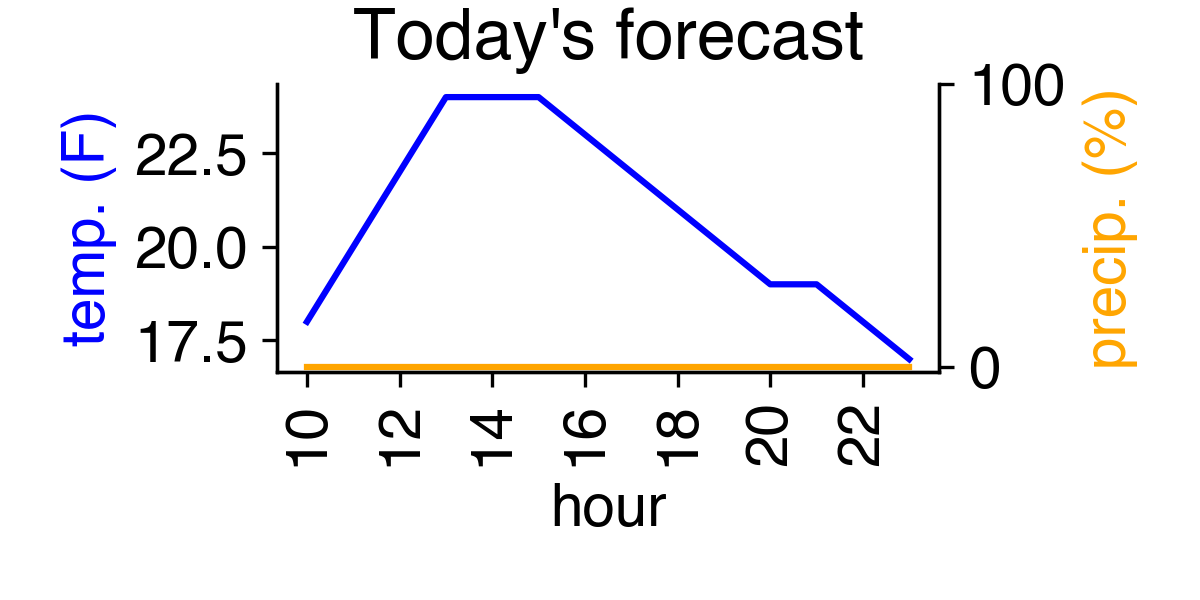
\includegraphics[width=1.0in]{images/forecast.png},\centerline{The Atom}] The \verb+multicol+ package allows using multiple columns without starting a new page.  Using floats is not possible in a columns environment, however with the \verb+picinpar+ package, I can set a picture inside a block of text---just like you one you see here.  Isn't \LaTeX{} cool?
And now we're just filling more space, and yet more space.  
\end{window}
\closearticle

\headline{Another Headline}
This is just an example to fill up some space, but as long as I have your attention, I'll give some newspaper advice.

I suppose we could also show how an equation is type set:
\begin{displaymath}
x=\frac{-b\pm\sqrt{b^2-4ac}}{2a}
\end{displaymath}
and there you have it.

\byline{Weather}{}
\closearticle

\headline{Sports}
% \lipsum[1]
\closearticle

\headline{Weather}

% \noindent\rule{\linewidth}{0.5pt}

\center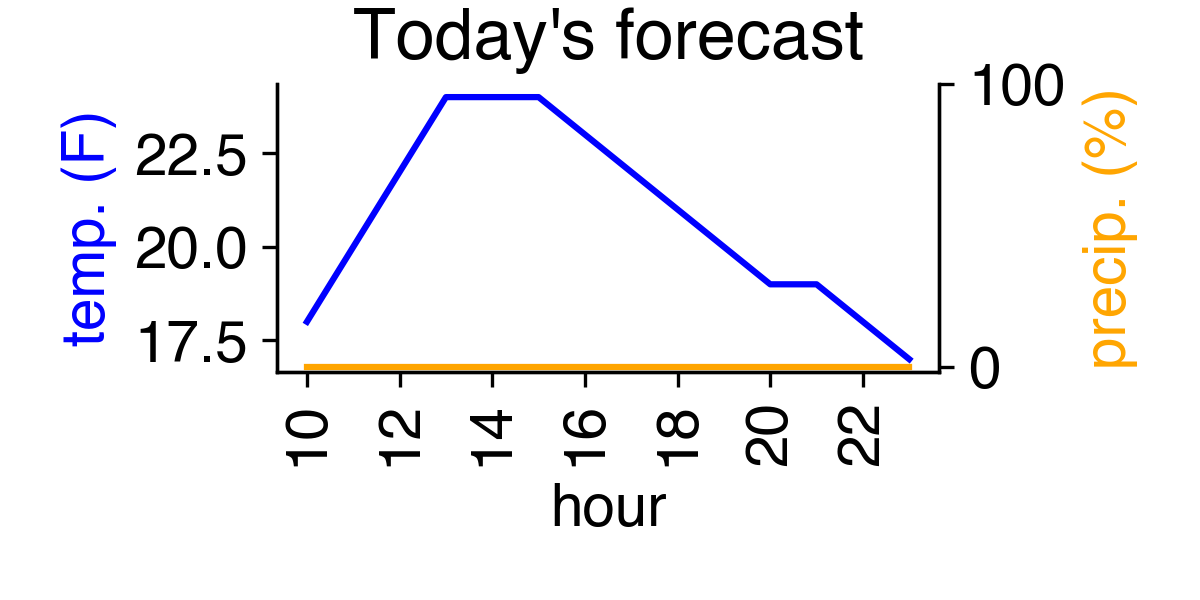
\includegraphics[width=\linewidth]{images/forecast.png}

\headline{Comics}
\center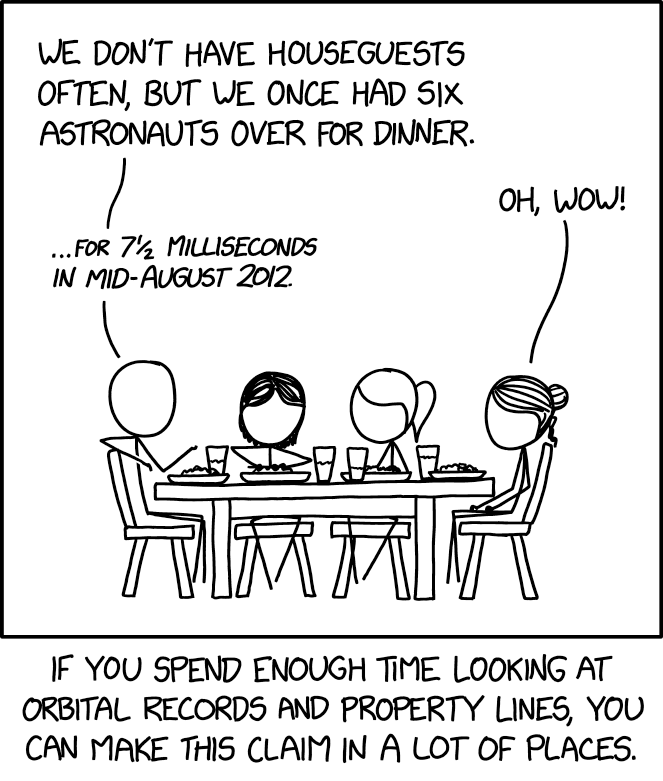
\includegraphics[width=\linewidth]{images/comic.png}
\closearticle

% \lipsum[1]

\headline{Games}
\vspace{-0.5cm}

Robin's Maze\vspace{-0.5cm}
\center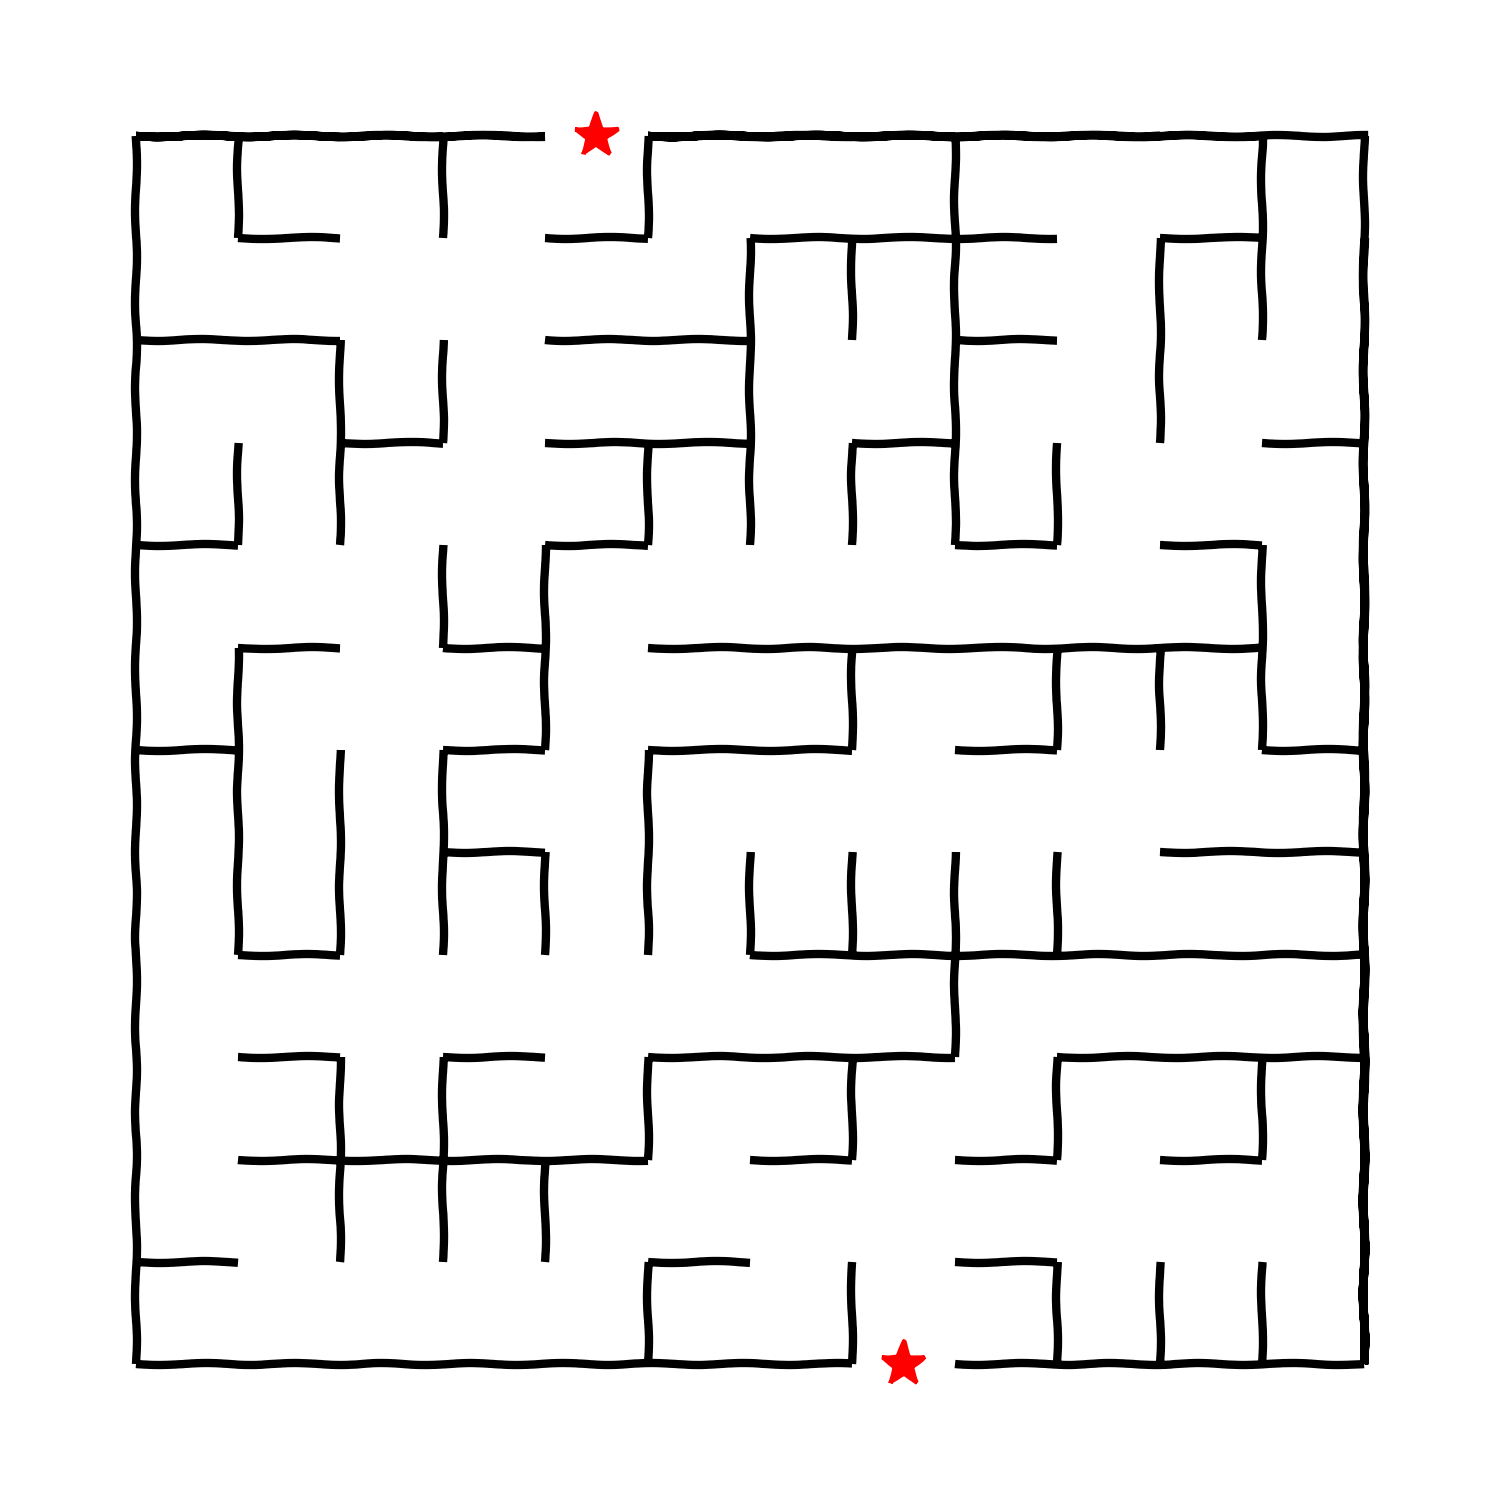
\includegraphics[width=\linewidth]{images/maze_r.png}

Jordan's Maze\vspace{-0.5cm}
\center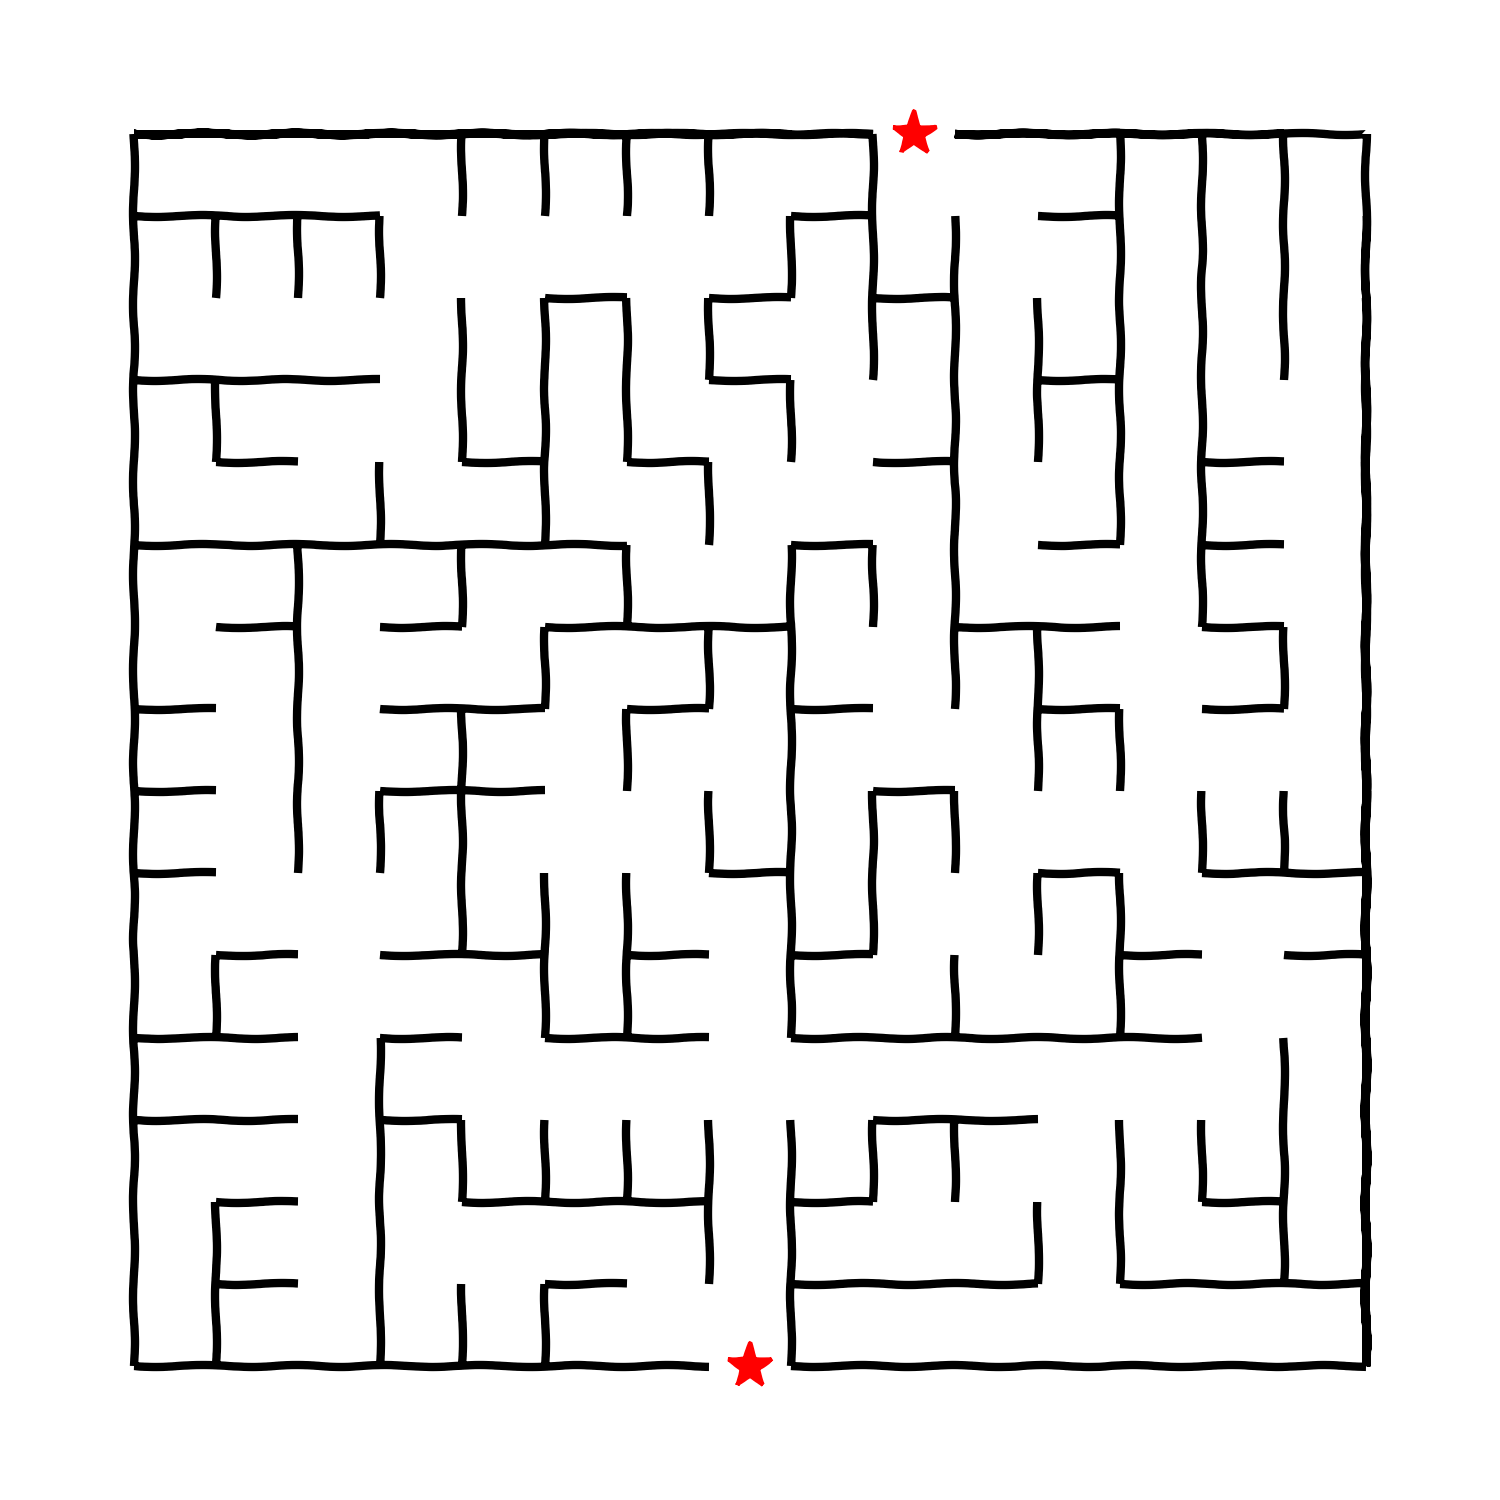
\includegraphics[width=\linewidth]{images/maze_j.png}

\renewcommand*\sudokuformat[1]{\sffamily#1}
\setlength\sudokusize{5cm}
\setlength\sudokuthickline{1pt}
Jess's Sudoku\vspace{0.2cm}
\begin{sudoku-block}
| |2| |4| | |7|9| |.
|6|5|4|7| |9| |3| |.
| |8|7| |2| |4| |5|.
|8|7| |5| |1|6|2|4|.
| |4| |9|7|8| |1| |.
|1| |5|6|4| | | |7|.
| | |2| |6|5|8|7| |.
|5| |3| |9| | |4|1|.
| | |8| | |4|3| |6|.
\end{sudoku-block}

\end{multicols}

\end{document}